\documentclass[11pt,a4paper]{article}

% --- Core Geometry & Typography ---
\usepackage[utf8]{inputenc}
\usepackage[margin=1in]{geometry}
\usepackage{amsmath,amssymb}
\usepackage{booktabs}
\usepackage{tabularx}
\usepackage{longtable}
\usepackage{array}
\usepackage{listings}
\usepackage{xcolor}
\usepackage[final]{graphicx}
\setkeys{Gin}{draft=false}
\usepackage{hyperref}
\usepackage{fancyhdr}
\usepackage{tikz}
\usetikzlibrary{shapes.geometric, arrows.meta, positioning}

% Supports imagesmilestone2 subfolder, relative path, and root directory lookup (Overleaf / TeX Live)
\graphicspath{{imagesmilestone2/}{./imagesmilestone2/}{./}}

% --- Custom Colors ---
\definecolor{infosysblue}{RGB}{58, 110, 184}
\definecolor{codegreen}{rgb}{0,0.6,0}
\definecolor{codegray}{rgb}{0.5,0.5,0.5}
\definecolor{codepurple}{rgb}{0.58,0,0.82}
\definecolor{backcolour}{rgb}{0.96,0.96,0.96}

% --- Header & Footer Formatting ---
\pagestyle{fancy}
\fancyhf{}
\lhead{\small BugTracker Milestone 2 Report}
\rhead{\small Infosys Springboard 7.0}
\cfoot{\small Page \thepage}
\renewcommand{\headrulewidth}{0.4pt}
\renewcommand{\footrulewidth}{0.4pt}

% --- Hyperlink Setup ---
\hypersetup{
    colorlinks=true,
    linkcolor=blue!70!black,
    citecolor=blue!70!black,
    urlcolor=blue!70!black
}

% --- Code Listing Settings ---
\lstdefinestyle{codeStyle}{
    backgroundcolor=\color{backcolour},   
    commentstyle=\color{codegreen},
    keywordstyle=\color{blue!80!black}\bfseries,
    numberstyle=\tiny\color{codegray},
    stringstyle=\color{codepurple},
    basicstyle=\ttfamily\footnotesize,
    breakatwhitespace=false,         
    breaklines=true,                 
    captionpos=b,                    
    keepspaces=true,                 
    numbers=none,                    
    numbersep=5pt,                  
    showspaces=false,                
    showstringspaces=false,
    showtabs=false,                  
    tabsize=2,
    frame=single,
    rulecolor=\color{black!20}
}
\lstset{style=codeStyle}

\begin{document}

% =========================================================================
% STANDALONE COVER PAGE
% =========================================================================
\begin{titlepage}
    \thispagestyle{empty}
    \centering
    \vspace*{3.5cm}

    {\large \textbf{\textcolor{infosysblue}{Infosys Springboard Virtual Internship 7.0}}}\\[2.2cm]

    {\Large \textbf{INTELLIGENT SOFTWARE DEFECT TRACKING\\[0.3em]
    SYSTEM WITH RESOLUTION ASSISTANCE}}\\[2.5cm]

    {\normalsize \textbf{MILESTONE 2 Report:}}\\[0.4em]
    {\normalsize \textbf{WORKFLOW AUTOMATION AND COLLABORATION}}\\[4cm]

    {\small Submitted By:}\\[0.3em]
    {\normalsize Ajay Kumar K R}\\[0.2em]
    {\small Batch 3 Intern}\\[1.6cm]

    {\small Submitted To:}\\[0.3em]
    {\normalsize Dr Sumathy S}\\[0.2em]
    {\small Infosys Springboard Mentor}

    \vfill
\end{titlepage}

\newpage

% =========================================================================
% 1. EXECUTIVE SUMMARY
% =========================================================================
\section{Executive Summary}
The Intelligent Software Defect Tracking System with Resolution Assistance (\textbf{BugTracker}) is a full-stack platform engineered to provide software engineering organizations with a centralized ecosystem for defect logging, automated triage, collaborative remediation, and Agile iteration governance. While foundational entities (user accounts, projects, basic defect records) were registered in initial iterations, software engineering in team environments requires structured coordination: objective prioritization rather than subjective triage, granular auditability, segregated role permissions, agile sprint iteration grouping, and automated lifecycle state machines.

Milestone 2 (Weeks 3--4) advances the platform from a foundational CRUD defect registry into a complete collaborative defect tracking and Agile project management platform. The platform is implemented via a decoupled three-tier architecture: a React 18 single-page application (TypeScript, Vite, Tailwind CSS) for the presentation layer, and an asynchronous FastAPI (Python 3.11) application core backed by PostgreSQL 16 and SQLAlchemy 2.0 (AsyncIO) for persistence, state machines, and business rules.

\subsection{Scope Covered in This Report}
\begin{itemize}
    \item \textbf{Mathematical Issue Prioritization}: Eliminating arbitrary priority tagging via the mentor-specified formula $\text{Priority Score} = \text{Severity Weight} \times \text{Category Urgency Weight}$.
    \item \textbf{Smart Assignee Recommendation Engine}: Automated triage recommendation analyzing issue semantics, historical velocity, and current developer workload balance.
    \item \textbf{Collaboration Primitives}: Threaded issue discussions, magic-byte validated multi-tier file attachments (PNG, JPEG, PDF), and real-time push alerts.
    \item \textbf{Forensic Immutable Audit Engine}: Append-only activity logging capturing client IP, user-agent, actor ID, and full JSONB before/after state diffs.
    \item \textbf{Agile Sprint Planning \& Capacity Management}: Iteration modeling, unassigned backlog defect allocation, and capacity estimation formulas.
    \item \textbf{Sprint Approval Governance}: Formal bi-directional sprint workflow requiring tester submission and administrative evaluation, prohibiting unauthorized self-approval.
    \item \textbf{Role-Based Access Control (RBAC)}: Dedicated workspaces and endpoint-level permission gating across User, Tester, and Admin roles.
    \item \textbf{Automated Test Verification}: Execution of 413 passing backend tests (Pytest 8.x) and clean production frontend build transpilation (Vite 5.4).
\end{itemize}

% =========================================================================
% 2. OBJECTIVE & SCOPE
% =========================================================================
\section{Objective \& Scope}
In software development teams, defect resolution frequently fails due to subjective triage, ambiguous ticket states, lack of verifiable audit trails, and untracked sprint commitments. Milestone 2 addresses these exact operational challenges by delivering an enterprise-ready collaboration and agile governance pipeline.

\subsection{User Roles \& Workspace Boundaries}
\begin{center}
\small
\begin{tabularx}{\textwidth}{lp{4cm}X}
\toprule
\textbf{Role} & \textbf{Workspace Route} & \textbf{Operational Capabilities} \\
\midrule
\texttt{USER} & \texttt{/dashboard}, \texttt{/issues} & Log defects, monitor reported tickets, confirm resolution (\texttt{CLOSED}), or reopen with mandatory justification. \\
\addlinespace
\texttt{TESTER} & \texttt{/tester-dashboard}, \texttt{/tester-sprints} & View assigned issues, advance defect lifecycle states, submit technical resolution summaries, begin work on sprints, and submit iterations for approval. \\
\addlinespace
\texttt{ADMIN} & \texttt{/admin-dashboard}, \texttt{/admin/sprints} & Global issue backlog triage, author sprint iterations, allocate unassigned tickets, assign dedicated QA specialists, evaluate/approve sprints, and manage users. \\
\bottomrule
\end{tabularx}
\end{center}

% =========================================================================
% 3. TECHNOLOGY STACK & ARCHITECTURE
% =========================================================================
\section{Technology Stack \& Architecture}

\subsection{Technology Stack Matrix}
\begin{center}
\small
\begin{tabularx}{\textwidth}{llX}
\toprule
\textbf{Layer} & \textbf{Technology} & \textbf{Version / Architectural Scope} \\
\midrule
Frontend Framework & React (TypeScript) & 18.x (SPA with Vite build tool) \\
UI / Styling & Tailwind CSS + Lucide & Modern dark-mode interface with Lucide icons \\
Frontend Routing & React Router DOM & v6 (Role-guarded workspace routing) \\
Data Visualization & Plotly.js & Interactive sprint velocity and defect charts \\
Backend Framework & FastAPI (Python) & Python 3.11, asynchronous REST API \\
ASGI Server & Uvicorn & High-performance asynchronous execution \\
Database Engine & PostgreSQL & 16 (Relational storage with JSONB support) \\
Database ORM & SQLAlchemy (AsyncIO) & 2.0 (Asynchronous sessions and unit of work) \\
Schema Validation & Pydantic & v2 (Request/response DTO serialization) \\
Real-Time Delivery & WebSockets & Starlette/FastAPI authenticated push channels \\
Security & PyJWT + bcrypt & HS256 stateless tokens with salted password hashing \\
Verification Suite & Pytest 8.x + pytest-asyncio & AsyncIO test harness and FastAPI TestClient \\
\bottomrule
\end{tabularx}
\end{center}

\subsection{Three-Tier Architecture Overview}
The BugTracker platform operates across three clean architectural tiers:
\begin{enumerate}
    \item \textbf{Presentation Tier}: Role-segregated workspaces (\texttt{USER}, \texttt{TESTER}, \texttt{ADMIN}) communicating via Axios with JWT request interceptors, supplemented by persistent WebSocket client listeners for immediate broadcast alerts.
    \item \textbf{Application Tier}: FastAPI core driving algorithmic defect prioritization, smart assignee matching, threaded comments, magic-byte attachment inspection, sprint lifecycle orchestration, and background push notification broadcasting.
    \item \textbf{Data Tier}: PostgreSQL relational database persisted via SQLAlchemy 2.0 AsyncIO ORM sessions, securing issues, project iterations, binary file metadata, immutable audit records, and notification logs.
\end{enumerate}

\subsection{Backend Project Structure}
\begin{lstlisting}[language=bash]
BugTracker/
|-- backend/
|   |-- app/
|   |   |-- core/          # Pydantic BaseSettings, configuration, security utils
|   |   |-- database/      # Async engine, sessionmaker, Base model declaration
|   |   |-- dependencies/  # JWT validation, role guards (require_role)
|   |   |-- models/        # SQLAlchemy ORM models (issues, sprints, audit, etc.)
|   |   |-- routes/        # FastAPI APIRouter modules (issues, sprints, comments)
|   |   |-- schemas/       # Pydantic validation models & payload schemas
|   |   |-- services/      # Domain business logic (smart_service, sprint_service)
|   |   |-- storage/       # UUID filesystem repository for verified attachments
|   |   `-- main.py        # Application root, CORS setup, router mounting
|   `-- tests/             # 19 Pytest test files (413 test cases)
`-- frontend/
    |-- src/
    |   |-- components/    # Reusable UI modals, navigation, and data tables
    |   |-- context/       # AuthContext and WebSocket notification context
    |   |-- pages/         # UserDashboard, TesterDashboard, AdminDashboard
    |   `-- services/      # Axios API clients and WebSocket connection handlers
\end{lstlisting}

% =========================================================================
% 4. POSTGRESQL DATABASE SCHEMA
% =========================================================================
\section{PostgreSQL Database Schema}

The relational data tier spans seven core tables in PostgreSQL 16, fully integrated with foreign keys, cascading rules, and specialized indexes for high-throughput querying.

\subsection{Schema Overview}
\begin{center}
\small
\begin{tabularx}{\textwidth}{lp{3.5cm}X}
\toprule
\textbf{Table Name} & \textbf{Primary Purpose} & \textbf{Key Architectural Relationships} \\
\midrule
\texttt{users} & Identity \& RBAC credentials & Referenced by reporters, assignees, authors, and uploaders. \\
\texttt{projects} & Project isolation scope & Parent boundary for sprints and issues. \\
\texttt{sprints} & Agile iterations \& capacity & Contains sprint dates, goals, review comments, and tester binding. \\
\texttt{issues} & Defect lifecycle \& prioritization & Core ticket record with severity, priority, category, and sprint foreign keys. \\
\texttt{issue\_comments} & Discussion threads & Cascade-deleted upon issue removal; linked to author JWT. \\
\texttt{issue\_attachments}& Binary asset tracking & Enforces 10MB limit, validated MIME type, and UUID file storage. \\
\texttt{audit\_logs} & Forensic immutable change trail & Append-only JSONB before/after diffs with network IP and actor ID. \\
\texttt{notifications} & Real-time push alert log & Recipient-indexed log driving in-app unread badges and WebSocket push. \\
\bottomrule
\end{tabularx}
\end{center}

\subsection{Table Specifications}

\subsubsection{Table: \texttt{issues} (Defect Record \& State Machine)}
\begin{lstlisting}[language=SQL]
CREATE TABLE issues (
    id SERIAL PRIMARY KEY,
    key VARCHAR(32) NOT NULL UNIQUE,
    title VARCHAR(255) NOT NULL,
    description TEXT,
    status VARCHAR(32) NOT NULL DEFAULT 'REPORTED',
    severity VARCHAR(32) NOT NULL DEFAULT 'MINOR',
    priority VARCHAR(32) NOT NULL DEFAULT 'MEDIUM',
    category VARCHAR(64),
    project_id INTEGER NOT NULL REFERENCES projects(id) ON DELETE CASCADE,
    reporter_id INTEGER NOT NULL REFERENCES users(id) ON DELETE RESTRICT,
    assignee_id INTEGER REFERENCES users(id) ON DELETE SET NULL,
    sprint_id INTEGER REFERENCES sprints(id) ON DELETE SET NULL,
    resolution_summary TEXT,
    resolved_at TIMESTAMPTZ,
    reopen_count INTEGER NOT NULL DEFAULT 0,
    reopen_reason TEXT,
    source VARCHAR(50) NOT NULL DEFAULT 'MANUAL',
    created_at TIMESTAMPTZ NOT NULL DEFAULT now(),
    updated_at TIMESTAMPTZ NOT NULL DEFAULT now()
);
CREATE UNIQUE INDEX ix_issues_key ON issues(key);
CREATE INDEX ix_issues_sprint_id ON issues(sprint_id);
\end{lstlisting}

\subsubsection{Table: \texttt{sprints} (Agile Iteration Governance)}
\begin{lstlisting}[language=SQL]
CREATE TABLE sprints (
    id SERIAL PRIMARY KEY,
    name VARCHAR(200) NOT NULL,
    goal TEXT,
    goal_status VARCHAR(50) NOT NULL DEFAULT 'NOT_STARTED',
    start_date TIMESTAMPTZ NOT NULL,
    end_date TIMESTAMPTZ NOT NULL,
    status VARCHAR(32) NOT NULL DEFAULT 'PLANNED',
    project_id INTEGER NOT NULL REFERENCES projects(id) ON DELETE CASCADE,
    assigned_tester_id INTEGER REFERENCES users(id) ON DELETE SET NULL,
    review_comment TEXT,
    submitted_at TIMESTAMPTZ,
    reviewed_at TIMESTAMPTZ,
    created_at TIMESTAMPTZ NOT NULL DEFAULT now(),
    updated_at TIMESTAMPTZ NOT NULL DEFAULT now()
);
\end{lstlisting}

\subsubsection{Table: \texttt{issue\_attachments} \& \texttt{issue\_comments}}
\begin{lstlisting}[language=SQL]
CREATE TABLE issue_comments (
    id SERIAL PRIMARY KEY,
    issue_id INTEGER NOT NULL REFERENCES issues(id) ON DELETE CASCADE,
    author_id INTEGER NOT NULL REFERENCES users(id) ON DELETE CASCADE,
    body TEXT NOT NULL,
    created_at TIMESTAMPTZ NOT NULL DEFAULT now(),
    updated_at TIMESTAMPTZ NOT NULL DEFAULT now()
);

CREATE TABLE issue_attachments (
    id SERIAL PRIMARY KEY,
    issue_id INTEGER NOT NULL REFERENCES issues(id) ON DELETE CASCADE,
    uploader_id INTEGER REFERENCES users(id) ON DELETE SET NULL,
    original_name VARCHAR(255) NOT NULL,
    stored_name VARCHAR(255) NOT NULL UNIQUE,
    file_path VARCHAR(512) NOT NULL,
    mime_type VARCHAR(100) NOT NULL,
    file_size_bytes INTEGER NOT NULL CHECK (file_size_bytes <= 10485760),
    created_at TIMESTAMPTZ NOT NULL DEFAULT now()
);
\end{lstlisting}

\subsubsection{Table: \texttt{audit\_logs} (Immutable Activity Trail)}
\begin{lstlisting}[language=SQL]
CREATE TABLE audit_logs (
    id SERIAL PRIMARY KEY,
    user_id INTEGER REFERENCES users(id) ON DELETE SET NULL,
    action VARCHAR(64) NOT NULL,
    entity_type VARCHAR(32) NOT NULL,
    entity_id INTEGER NOT NULL,
    old_values JSONB,
    new_values JSONB,
    ip_address VARCHAR(45),
    user_agent VARCHAR(255),
    created_at TIMESTAMPTZ NOT NULL DEFAULT now()
);
CREATE INDEX ix_audit_logs_entity ON audit_logs(entity_type, entity_id);
CREATE INDEX ix_audit_logs_created_at_desc ON audit_logs(created_at DESC);
\end{lstlisting}

% =========================================================================
% 5. DEFECT PRIORITIZATION & TRIAGE ENGINE
% =========================================================================
\section{Issue Prioritization \& Classification Engine}

A recurring breakdown in defect tracking is subjective triage: reporters arbitrarily classify minor issues as critical. Milestone 2 implements an objective, mathematical scoring engine evaluated deterministically.

\subsection{Mathematical Scoring Formula}
Implemented in \texttt{backend/app/services/smart\_service.py}, the engine computes priority:
\begin{equation}
\text{Priority Score} = \text{Severity Weight} \times \text{Category Urgency Weight}
\end{equation}

\subsection{Taxonomy Weights \& Operational Tiers}
\begin{itemize}
    \item \textbf{Severity Weights}: \texttt{CRITICAL} ($=4$), \texttt{MAJOR} ($=3$), \texttt{MINOR} ($=2$), \texttt{TRIVIAL} ($=1$).
    \item \textbf{Category Urgency Weights}:
    \begin{itemize}
        \item \textbf{High Urgency (Weight $=3$)}: \texttt{Security}, \texttt{Database} (Threatens data integrity, confidentiality, and ACID guarantees).
        \item \textbf{Medium Urgency (Weight $=2$)}: \texttt{API}, \texttt{Backend} (Disrupts integration layers and server services).
        \item \textbf{Low Urgency (Weight $=1$)}: \texttt{UI}, \texttt{Colors}, \texttt{Typo}, \texttt{Frontend} (Cosmetic presentation errors).
    \end{itemize}
    \item \textbf{Operational Priority Mapping}:
    \begin{equation}
        \text{Priority Tier} = 
        \begin{cases}
            \mathbf{URGENT}, & \text{if Score} \ge 10 \quad (\text{SLA: Immediate hotfix } \le 4\text{ hours}) \\
            \mathbf{HIGH},   & \text{if } 7 \le \text{Score} \le 9 \quad (\text{SLA: Active sprint } \le 24\text{ hours}) \\
            \mathbf{MEDIUM}, & \text{if } 4 \le \text{Score} \le 6 \quad (\text{SLA: Scheduled in upcoming sprint}) \\
            \mathbf{LOW},    & \text{if Score} < 4 \quad (\text{SLA: Routine maintenance})
        \end{cases}
    \end{equation}
\end{itemize}

\subsection{Smart Developer Assignee Matcher}
Exposed at \texttt{GET /issues/\{id\}/suggest-assignee}, this recommendation engine analyzes incoming defects to determine optimal developer allocation:
\begin{enumerate}
    \item \textbf{Keyword Extraction}: Parses title and description text using regex tokenizers to extract domain tokens (\texttt{auth}, \texttt{security}, \texttt{sql}, \texttt{api}, \texttt{ui}, \texttt{react}).
    \item \textbf{Competency Evaluation}: Inspects historical resolution logs in PostgreSQL to measure each developer's track record across matching categories.
    \item \textbf{Workload Balancing}: Computes open work-in-progress (WIP) counts. Developers carrying heavy active loads receive penalties, preventing team bottlenecks.
    \item \textbf{Ranked Output}: Emits the top 3 ranked developers with match percentages and explicit rationales.
\end{enumerate}

% =========================================================================
% 6. COMPLETE ISSUE LIFECYCLE & STATE MACHINE
% =========================================================================
\section{Defect Reporting \& Issue Lifecycle Management}

Defects follow a rigid, validated state machine preventing illegal lifecycle transitions:

\begin{center}
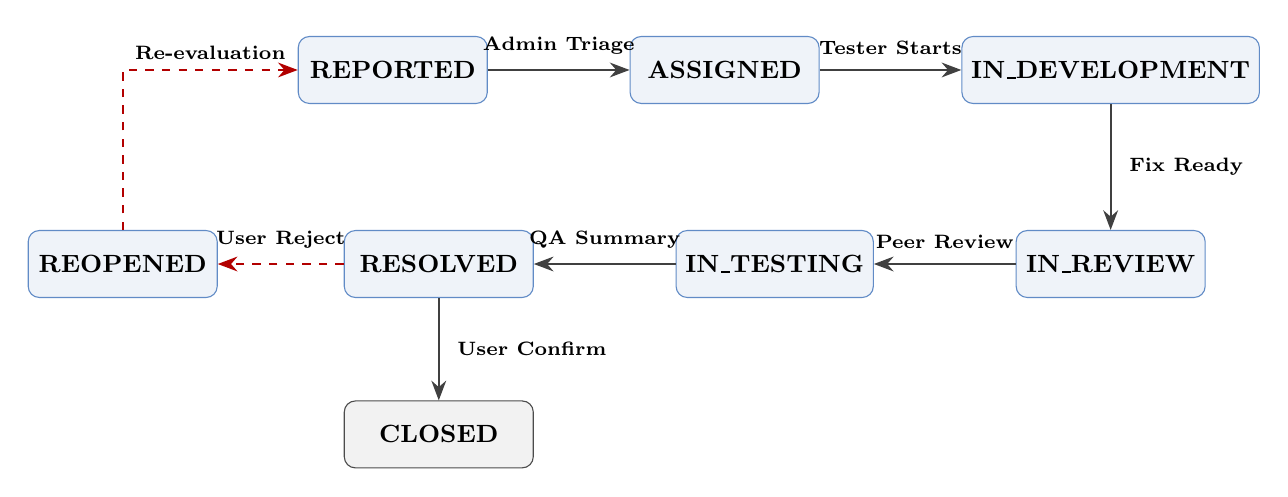
\begin{tikzpicture}[
    node distance=1.4cm and 1.8cm,
    state/.style={
        rectangle, 
        draw=infosysblue!80, 
        fill=infosysblue!8, 
        rounded corners=4pt, 
        minimum height=0.85cm, 
        minimum width=2.4cm, 
        font=\small\bfseries,
        align=center
    },
    terminal/.style={
        rectangle, 
        draw=black!70, 
        fill=black!5, 
        rounded corners=4pt, 
        minimum height=0.85cm, 
        minimum width=2.4cm, 
        font=\small\bfseries,
        align=center
    },
    edge/.style={->, >={Stealth[length=2.5mm]}, thick, draw=black!75},
    feedback/.style={->, >={Stealth[length=2.5mm]}, thick, dashed, draw=red!70!black}
]
    % Row 1: Intake & Development (Left to Right)
    \node[state] (rep) {REPORTED};
    \node[state, right=1.8cm of rep] (ass) {ASSIGNED};
    \node[state, right=1.8cm of ass] (dev) {IN\_DEVELOPMENT};

    % Row 2: Verification (Right to Left)
    \node[state, below=1.6cm of dev] (rev) {IN\_REVIEW};
    \node[state, left=1.8cm of rev] (tst) {IN\_TESTING};
    \node[state, left=1.8cm of tst] (res) {RESOLVED};

    % Row 3: Outcomes
    \node[state, left=1.6cm of res] (reo) {REOPENED};
    \node[terminal, below=1.3cm of res] (cls) {CLOSED};

    % Lifecycle Forward Edges
    \draw[edge] (rep) -- node[above=2pt, font=\scriptsize\bfseries]{Admin Triage} (ass);
    \draw[edge] (ass) -- node[above=2pt, font=\scriptsize\bfseries]{Tester Starts} (dev);
    \draw[edge] (dev) -- node[right=3pt, font=\scriptsize\bfseries]{Fix Ready} (rev);
    \draw[edge] (rev) -- node[above=2pt, font=\scriptsize\bfseries]{Peer Review} (tst);
    \draw[edge] (tst) -- node[above=2pt, font=\scriptsize\bfseries]{QA Summary} (res);
    
    % Resolution Outcomes (No Overlapping Lines)
    \draw[edge] (res) -- node[right=3pt, font=\scriptsize\bfseries]{User Confirm} (cls);
    \draw[feedback] (res) -- node[above=2pt, font=\scriptsize\bfseries]{User Reject} (reo);
    \draw[feedback] (reo.north) |- node[above, font=\scriptsize\bfseries, pos=0.75]{Re-evaluation} (rep.west);
\end{tikzpicture}
\end{center}

\subsection{State Transition Validation Rules}
\begin{center}
\small
\begin{tabularx}{\textwidth}{ccp{2.2cm}p{2.8cm}X}
\toprule
\textbf{Seq} & \textbf{Initial State} & \textbf{Permitted Role} & \textbf{Target State} & \textbf{Enforced Validation Criteria} \\
\midrule
1 & (Intake) & USER / ADMIN & \texttt{REPORTED} & Reporter bound from JWT; assignee set to NULL. \\
2 & \texttt{REPORTED} & ADMIN & \texttt{ASSIGNED} & Assignee must hold TESTER or DEVELOPER role. \\
3 & \texttt{ASSIGNED} & TESTER & \texttt{IN\_DEVELOPMENT} & Requester must match the assigned user ID. \\
4 & \texttt{IN\_DEV} & TESTER & \texttt{IN\_REVIEW} & Functional fix complete; peer review pending. \\
5 & \texttt{IN\_REVIEW} & TESTER & \texttt{IN\_TESTING} & Deployed to verification environment. \\
6 & \texttt{IN\_TESTING}& TESTER & \texttt{RESOLVED} & Requires \texttt{resolution\_summary} ($\ge 10$ chars). \\
7a & \texttt{RESOLVED} & USER & \texttt{CLOSED} & Original reporter confirms fix remediation. \\
7b & \texttt{RESOLVED} & USER / ADMIN & \texttt{REOPENED} & Requires mandatory \texttt{reopen\_reason} ($\ge 5$ chars). \\
\bottomrule
\end{tabularx}
\end{center}

% =========================================================================
% 7. SPRINT PLANNING & GOVERNANCE
% =========================================================================
\section{Sprint Planning \& Approval Governance}

Milestone 2 bundles defect remediation into Agile delivery iterations governed by managerial approval.

\subsection{Capacity Modeling \& Backlog Triage}
Sprints group defects under delivery milestones. Iteration bandwidth is evaluated using:
\begin{equation}
\text{Total Available Hours} = \text{Estimated Team Members} \times \text{Working Days} \times \text{Hours Per Day}
\end{equation}
As illustrated in Figure~\ref{fig:create_sprint}, the sprint creation interface captures iteration parameters, scheduled delivery bounds, and team capacity inputs to prevent overallocation.

\begin{figure}[htbp]
\centering
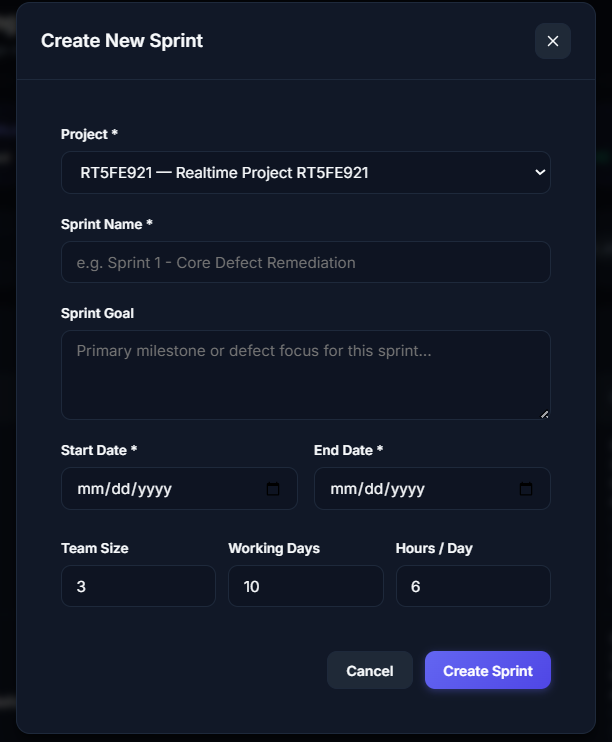
\includegraphics[width=0.55\textwidth]{imagesmilestone2/create_new_sprints.png}
\caption{Create New Sprint modal showing iteration authoring fields, scheduled dates, and capacity inputs (team size: 3 members, duration: 10 working days, effort: 6 hrs/day).}
\label{fig:create_sprint}
\end{figure}

Unassigned issues (\texttt{sprint\_id IS NULL}), including Kaggle ISEC benchmark defects (\texttt{source = 'KAGGLE\_ISEC'}), remain in the project backlog until an administrator triages them via \texttt{PATCH /sprints/\{id\}/issues}. Figure~\ref{fig:sprints_planning} depicts the central Agile administration console managing active sprints, tester bindings, and backlog linkage.

\begin{figure}[htbp]
\centering
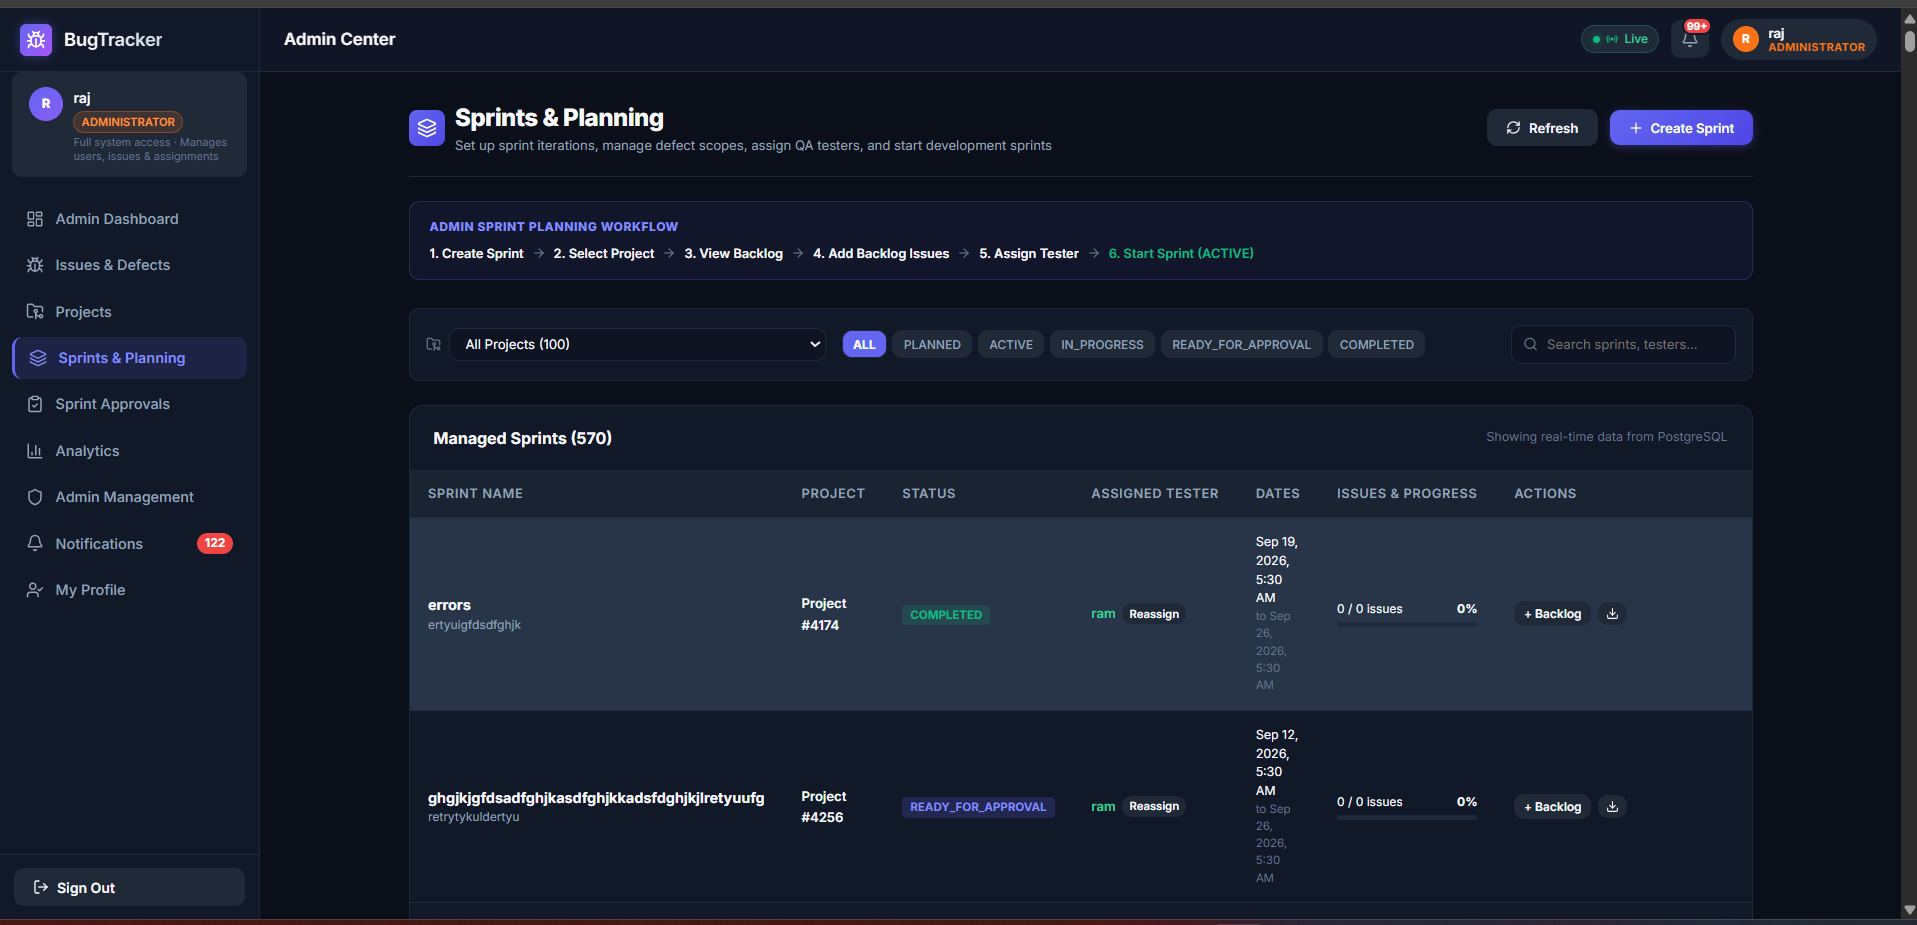
\includegraphics[width=0.95\textwidth]{imagesmilestone2/sprints_and_planning.png}
\caption{Admin Sprints and Planning console displaying managed sprints, lifecycle statuses (\texttt{COMPLETED}, \texttt{READY\_FOR\_APPROVAL}), tester assignments, and backlog linkage.}
\label{fig:sprints_planning}
\end{figure}

\subsection{Sprint Approval State Machine}
\begin{center}
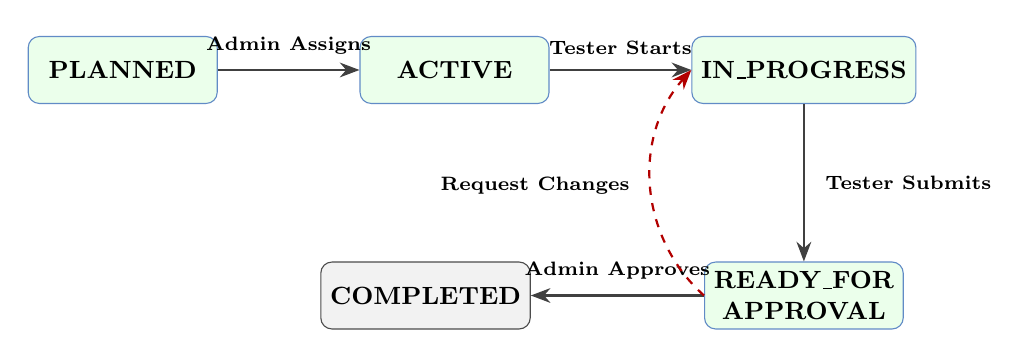
\begin{tikzpicture}[
    node distance=1.6cm and 2.0cm,
    state/.style={
        rectangle, 
        draw=infosysblue!80, 
        fill=green!8, 
        rounded corners=4pt, 
        minimum height=0.85cm, 
        minimum width=2.4cm, 
        font=\small\bfseries, 
        align=center
    },
    approved/.style={
        rectangle, 
        draw=black!70, 
        fill=black!5, 
        rounded corners=4pt, 
        minimum height=0.85cm, 
        minimum width=2.4cm, 
        font=\small\bfseries, 
        align=center
    },
    edge/.style={->, >={Stealth[length=2.5mm]}, thick, draw=black!75},
    feedback/.style={->, >={Stealth[length=2.5mm]}, thick, dashed, draw=red!70!black}
]
    \node[state] (pla) {PLANNED};
    \node[state, right=1.8cm of pla] (act) {ACTIVE};
    \node[state, right=1.8cm of act] (inp) {IN\_PROGRESS};
    \node[state, below=2.0cm of inp] (rfa) {READY\_FOR\\APPROVAL};
    \node[approved, left=2.2cm of rfa] (com) {COMPLETED};

    \draw[edge] (pla) -- node[above=2pt, font=\scriptsize\bfseries]{Admin Assigns} (act);
    \draw[edge] (act) -- node[above=2pt, font=\scriptsize\bfseries]{Tester Starts} (inp);
    \draw[edge] (inp) -- node[right=4pt, font=\scriptsize\bfseries]{Tester Submits} (rfa);
    \draw[edge] (rfa) -- node[above=2pt, font=\scriptsize\bfseries]{Admin Approves} (com);
    \draw[feedback] (rfa.west) to[bend left=45] node[left=4pt, font=\scriptsize\bfseries]{Request Changes} (inp.west);
\end{tikzpicture}
\end{center}

\subsection{Governance Invariants}
\begin{enumerate}
    \item \textbf{Assignment Invariant}: Only an \texttt{ADMIN} can transition a sprint from \texttt{PLANNED} to \texttt{ACTIVE} by assigning a dedicated tester.
    \item \textbf{Execution Invariant}: Only the assigned \texttt{TESTER} can acknowledge assignment via \texttt{POST /sprints/\{id\}/begin-work} to transition to \texttt{IN\_PROGRESS}.
    \item \textbf{Submission Invariant}: Transitioning to \texttt{READY\_FOR\_APPROVAL} requires the sprint to be actively \texttt{IN\_PROGRESS}. Direct jumps from \texttt{ACTIVE} are rejected (\texttt{HTTP 400 Bad Request}).
    \item \textbf{Approval Boundary}: Testers are barred from self-approving sprints (\texttt{HTTP 403 Forbidden}). Only administrators may sign off (\texttt{COMPLETED}) or request changes with mandatory feedback commentary.
\end{enumerate}

As depicted in Figure~\ref{fig:sprints_approvals}, iterations submitted by testers enter the managerial review queue, where administrators evaluate delivery artifacts before either approving or requesting rework.

\begin{figure}[htbp]
\centering
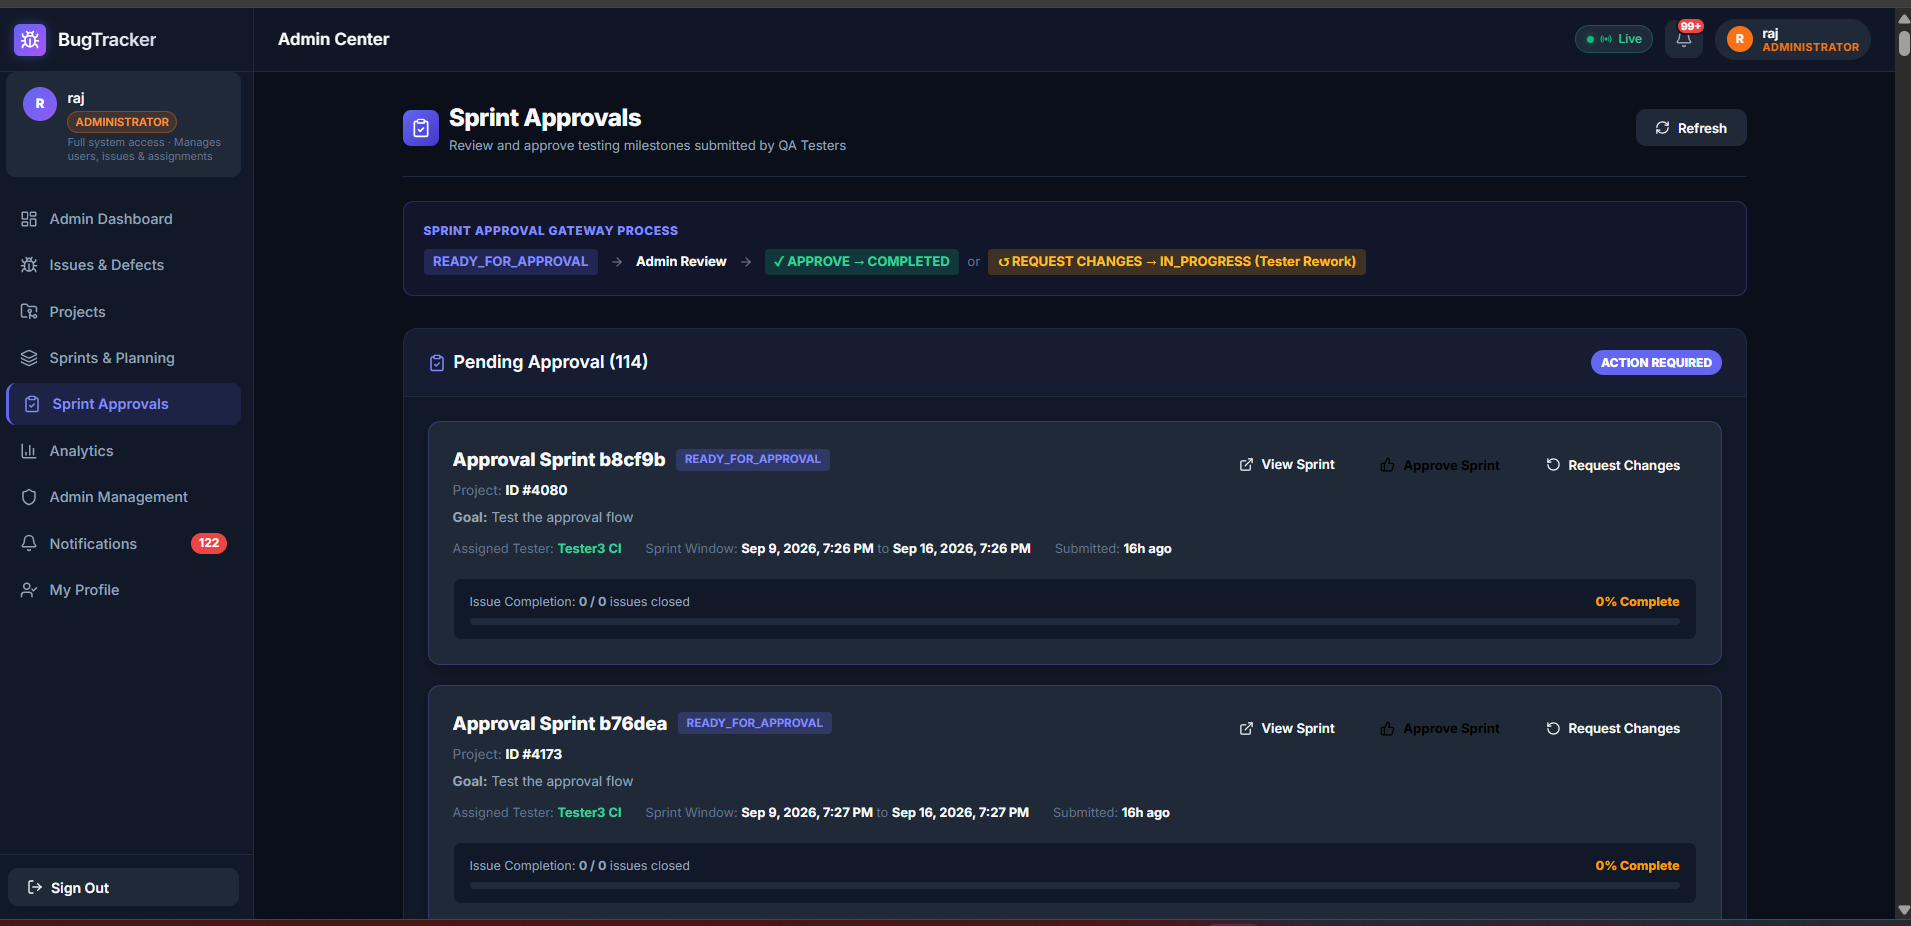
\includegraphics[width=0.95\textwidth]{imagesmilestone2/sprints_approvals.png}
\caption{Admin Sprint Approvals console displaying pending iterations in \texttt{READY\_FOR\_APPROVAL} state with direct Approve and Request Changes governance controls.}
\label{fig:sprints_approvals}
\end{figure}

% =========================================================================
% 8. COLLABORATION SUBSYSTEM & AUDIT LOGGING
% =========================================================================
\section{Collaboration Subsystem: Comments, Attachments \& Audits}

\subsection{Threaded Comments}
Comments are persisted in \texttt{issue\_comments}. The author identity is extracted exclusively from the validated JWT token, preventing author spoofing. Cascading deletes (\texttt{ON DELETE CASCADE}) ensure child comments are removed if a defect is purged.

\subsection{Multi-Tiered Secure Attachment Pipeline}
Binary uploads are processed through a hardened verification sequence:
\begin{itemize}
    \item \textbf{Payload Ceiling}: Strict 10 MB limit ($10,485,760$ bytes) enforced at the reverse proxy and FastAPI layer.
    \item \textbf{Extension Blacklist}: Executable extensions are rejected outright (\texttt{.exe}, \texttt{.bat}, \texttt{.sh}, \texttt{.dll}, \texttt{.bin}, \texttt{.msi}).
    \item \textbf{Magic-Byte Stream Inspection}: The server reads the initial bytes of the stream to confirm valid MIME signatures:
    \begin{itemize}
        \item PNG: \texttt{\textbackslash x89PNG\textbackslash r\textbackslash n\textbackslash x1a\textbackslash n}
        \item JPEG: \texttt{\textbackslash xff\textbackslash xd8\textbackslash xff}
        \item PDF: \texttt{\%PDF}
    \end{itemize}
    \item \textbf{Storage Isolation}: Filenames are replaced with sanitized UUID v4 identifiers, mitigating directory traversal risks (\texttt{../../etc/passwd}).
\end{itemize}

\subsection{Immutable Audit Engine}
All lifecycle changes emit an \texttt{AuditLog} record capturing:
\begin{itemize}
    \item Point-in-time entity state before mutation (\texttt{old\_values} JSONB).
    \item Point-in-time entity state following mutation (\texttt{new\_values} JSONB).
    \item Client network IP (IPv4/IPv6) and HTTP \texttt{User-Agent}.
    \item Immutability guarantee: The backend exposes zero \texttt{PUT}, \texttt{PATCH}, or \texttt{DELETE} endpoints for audit records.
\end{itemize}

% =========================================================================
% 9. REAL-TIME NOTIFICATIONS & ROLE MATRIX
% =========================================================================
\section{Role Authorization Matrix \& Real-Time Notifications}

\subsection{Role-Based Access Control (RBAC) Matrix}
\begin{center}
\small
\begin{tabularx}{\textwidth}{lcccc}
\toprule
\textbf{Operational Capability} & \textbf{USER} & \textbf{TESTER} & \textbf{DEVELOPER} & \textbf{ADMIN} \\
\midrule
Report Defects / View Own & Yes & Yes & Yes & Yes \\
Confirm Resolution (\texttt{CLOSED}) & Yes & No & No & Yes \\
Reopen Defect (with reason) & Yes & Yes* & No & Yes \\
Advance Defect Lifecycle States & No & Yes & Yes & No \\
Submit Resolution Summary & No & Yes & Yes & No \\
Access Tester Workspaces & No & Yes & Yes & No \\
Execute Sprint ``Begin Work'' & No & Yes & Yes & No \\
Submit Sprint for Approval & No & Yes & Yes & No \\
Create Projects \& Sprints & No & No & No & Yes \\
Assign QA Specialists & No & No & No & Yes \\
Approve / Request Sprint Changes & No & No & No & Yes \\
Manage Users \& System Analytics & No & No & No & Yes \\
\bottomrule
\end{tabularx}
\end{center}
\vspace{-0.5em}
\noindent\footnotesize{*Testers may reopen issues assigned to them or originally submitted by them.}

Figure~\ref{fig:tester_sprints} illustrates the dedicated tester workspace interface, where assigned sprint iterations, review progress, and report generation actions are coordinated.

\begin{figure}[htbp]
\centering
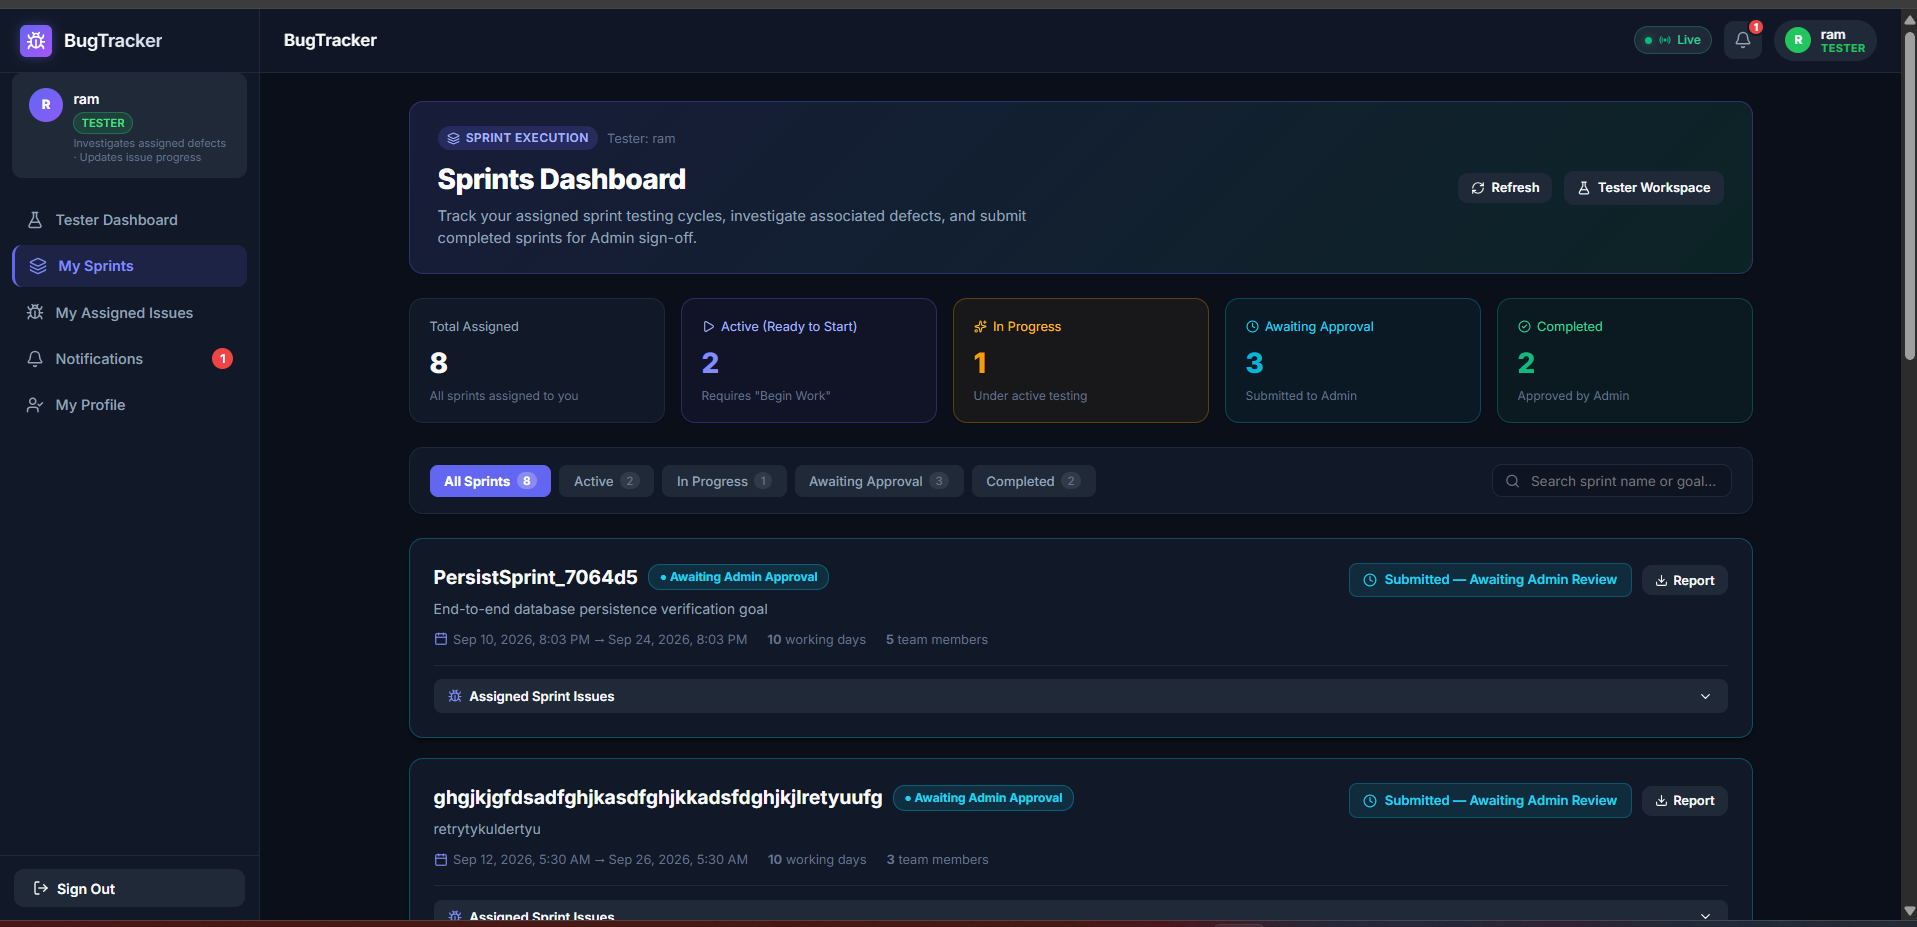
\includegraphics[width=0.95\textwidth]{imagesmilestone2/tester_sprints.png}
\caption{Tester Workspace Sprints Dashboard showing assigned iterations across active states, submission statuses, and direct report generation actions.}
\label{fig:tester_sprints}
\end{figure}

\subsection{WebSocket Push Notification Architecture}
The system serves an authenticated WebSocket line at \texttt{/ws/notifications/\{user\_id\}?token=\{jwt\}}. Actions like defect assignments, review requests, and approvals trigger FastAPI background tasks that commit a database notification and broadcast a structured JSON payload:
\begin{lstlisting}[language=json]
{
  "type": "notification",
  "data": {
    "id": 104,
    "notification_type": "ISSUE_ASSIGNED",
    "title": "Defect Assigned",
    "message": "You have been assigned to defect BUG-204.",
    "entity_type": "ISSUE",
    "entity_id": 204,
    "entity_key": "BUG-204",
    "created_at": "2026-09-08T18:30:00Z"
  }
}
\end{lstlisting}

% =========================================================================
% 10. TESTING RESULTS & SCREENSHOTS
% =========================================================================
\section{Verification \& Performance Reports}

\subsection{Agile Velocity \& Capacity Reports}
Figures \ref{fig:admin_report} and \ref{fig:tester_report} illustrate the generated Agile sprint execution reports for both management evaluation and QA validation.

\begin{figure}[htbp]
\centering
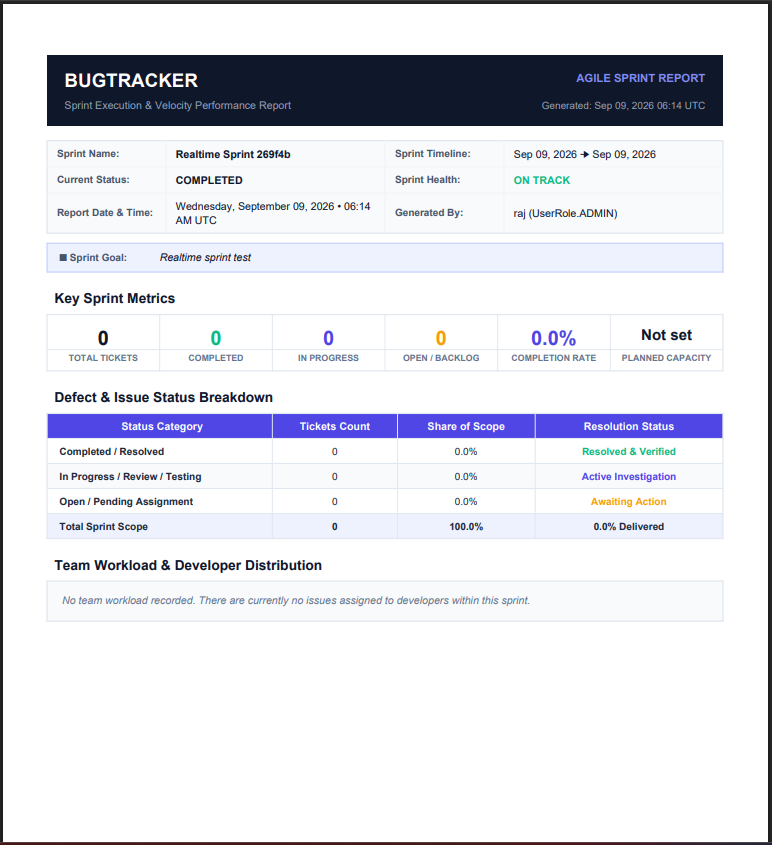
\includegraphics[width=0.82\textwidth]{imagesmilestone2/report_of_sprints.png}
\caption{Agile Sprint Execution \& Velocity Performance Report generated for an administrator, detailing sprint metrics, completion rate, and defect status breakdown.}
\label{fig:admin_report}
\end{figure}

\begin{figure}[htbp]
\centering
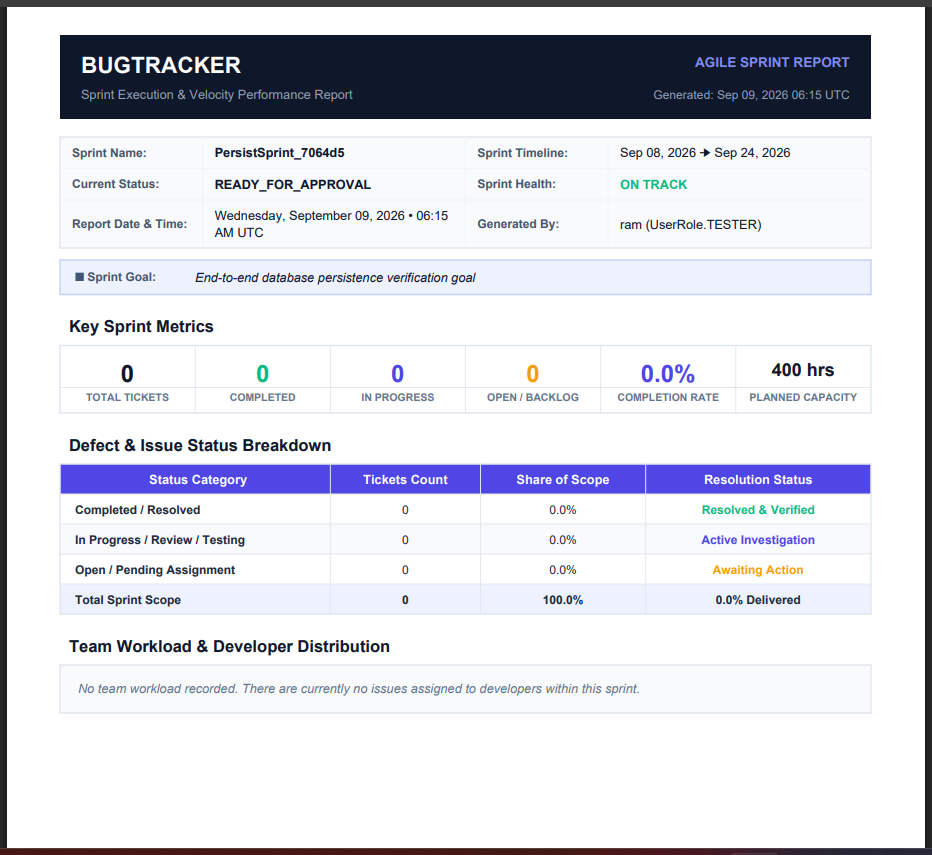
\includegraphics[width=0.82\textwidth]{imagesmilestone2/report_of_tester_sprint.png}
\caption{Agile Sprint Performance Report generated from the Tester workspace displaying planned capacity (400 hrs), timeline bounds, and delivery metrics.}
\label{fig:tester_report}
\end{figure}

\subsection{Automated Test Verification}
The test suite was executed across 19 Pytest modules using \texttt{pytest-asyncio}:
\begin{lstlisting}[language=bash]
$ python -m pytest -v
================== 413 passed, 11 skipped, 3 warnings in 36.66s ==================
\end{lstlisting}
\begin{itemize}
    \item \textbf{Full Workflow Assertion}: \texttt{test\_e2e\_workflow.py} asserts the complete loop: User reports $\rightarrow$ Admin triages $\rightarrow$ Tester resolves $\rightarrow$ User confirms $\rightarrow$ User reopens.
    \item \textbf{Sprint Governance Assertion}: \texttt{test\_sprint\_approval.py} asserts \texttt{HTTP 403} on self-approval attempts, \texttt{HTTP 400} on illegal state jumps, and validates rework cycles.
    \item \textbf{Data Durability}: \texttt{test\_sprint\_persistence.py} verifies physical PostgreSQL commits and constraint validation using raw SQL executions.
    \item \textbf{Frontend Production Transpilation}: Vite 5.4 build transformed 2,936 modules with \textbf{0 Errors} in 20.46s.
\end{itemize}

% =========================================================================
% 11. DELIVERABLES & OUTCOME MATRIX
% =========================================================================
\section{Deliverables \& Acceptance Criteria}

\begin{center}
\small
\begin{tabularx}{\textwidth}{p{9.5cm}c}
\toprule
\textbf{Program Acceptance Criterion} & \textbf{Status} \\
\midrule
Deterministic Priority Formula ($\text{Severity} \times \text{Category}$) with 4 Operational Tiers & Complete \\
Smart Assignee Matcher analyzing developer velocity, competencies, and active WIP & Complete \\
Threaded defect discussion stream with JWT-enforced author identity & Complete \\
Multi-tiered attachment pipeline (10MB cap, magic-byte inspection, executable blocking) & Complete \\
Immutable, append-only forensic audit engine with PostgreSQL JSONB field diffs & Complete \\
Asynchronous WebSocket real-time push gateway with zero polling overhead & Complete \\
Agile sprint authoring, capacity estimation, and unassigned backlog issue allocation & Complete \\
Bi-directional sprint approval state machine preventing unauthorized self-approval & Complete \\
Role-Based Access Control enforcing distinct workspaces (User, Tester, Admin) & Complete \\
Automated test suite passing with zero failures across 19 modules (413 tests) & Complete \\
Frontend production build transpilation with zero TypeScript compiler errors & Complete \\
\bottomrule
\end{tabularx}
\end{center}

% =========================================================================
% 12. CONCLUSION & ROADMAP
% =========================================================================
\section{Conclusion \& Future Roadmap}
Milestone 2 establishes BugTracker as a comprehensive collaborative defect tracking and Agile iteration platform. By integrating mathematical prioritization, role-governed state machines, secure binary attachments, forensic audit trails, and real-time push messaging, the system eliminates communication bottlenecks and operational ambiguity across software quality assurance lifecycles.

\subsection{Future Roadmap (Milestone 3 Preview)}
\begin{itemize}
    \item \textbf{AI-Assisted Resolution Engine}: Fine-tuning Large Language Models on Kaggle ISEC defect datasets to generate automated code remediation suggestions.
    \item \textbf{Automated Defect Clustering}: Utilizing semantic vector embeddings to group related tickets and detect duplicate regression patterns.
    \item \textbf{Containerized Cloud Orchestration}: Full Docker Compose and Kubernetes deployment automation with end-to-end TLS termination.
\end{itemize}

\vspace{1.5em}
\noindent\textbf{Submitted by:}\\
Ajay Kumar K R -- Infosys Springboard Virtual Internship 7.0 (Batch 3)

\end{document}
